%
\documentclass[hyperref,compress,handout,9pt,usepdftitle=false]{beamer}


%% Version: 2016-05-13
%% common packages
\usefonttheme[onlymath]{serif} % apply Serif font to math
\usepackage[USenglish]{babel}
\usepackage{amsbsy}
\usepackage{mathtools}
\usepackage{graphicx}
\usepackage{subfigure}
\usepackage{color}
\usepackage{booktabs}
\usepackage{wasysym} % wasy fonts, see texdoc.net/texmf-dist/doc/latex/wasysym/wasysym.pdf
\usepackage{lmodern} % to avoid font size not available warning
\usepackage{textcomp} % to avoid font warning for textbullet used in \item

%% to allow citation as footnote
\usepackage{natbib}
% and to reduce footnote font size
\usepackage{etoolbox}
\makeatletter
\patchcmd{\@makefntext}{\insertfootnotetext{#1}}{\insertfootnotetext{\scriptsize#1}}{}{}
\makeatother


%% macros for commenting
\usepackage[normalem]{ulem} % to use \sout
\newcommand{\cut}[1]{{}}
\newcommand{\remove}[1]{{\color{Gray}\sout{#1}}}
\newcommand{\revise}[1]{{\color{blue}#1}}
\newcommand{\commwy}[1]{{\color{red}(wy: #1)}} % Wotao Yin

\newcommand{\code}[1]{\texttt{#1}}


%% template for beamer

\mode<presentation>
{
  % background and theme
  \setbeamertemplate{background canvas}[vertical shading][bottom=white!10,top=white!10]
  \usetheme{default}

  % page number
  %\setbeamertemplate{footline}{\insertframenumber/\inserttotalframenumber}
  \setbeamertemplate{footline}[frame number]

  % section in table of contents has numbers
  \setbeamertemplate{sections/subsections in toc}[sections numbered]

  % no navigation bottoms
  \setbeamertemplate{navigation symbols}{}

  % itemize, black bullet, %150 spacing between items using "witemize"
  \setbeamertemplate{itemize items}[circle]
  \setbeamercolor{itemize item}{fg=black}
  \setbeamercolor{enumerate item}{fg=black}
  \setbeamercolor{itemize subitem}{fg=black}
  \setbeamercolor{enumerate subitem}{fg=black}
  \newenvironment{witemize}{\itemize\addtolength{\itemsep}{0.3\baselineskip}}{\enditemize}

  % itemize enumerate use normal sized texts
  \setbeamertemplate{itemize/enumerate body begin}{\normalsize}
  \setbeamertemplate{itemize/enumerate subbody begin}{\normalsize}
  \setbeamertemplate{itemize/enumerate subsubbody begin}{\normalsize}

  % block, black over gray with no shadow
  \setbeamertemplate{blocks}[rounded][shadow=false]
  \setbeamercolor{block title}{fg=black,bg=gray!40}
  \setbeamercolor{block body}{fg=black,bg=gray!10}

  % frametitle, bold, black, centered
  \setbeamertemplate{frametitle}[default][center]
  \setbeamercolor{frametitle}{fg=black}
  \setbeamerfont{frametitle}{shape=\bfseries}

  % line spacing
  \linespread{1.2}

  \setlength{\parskip}{\smallskipamount}
}

%% macros for letters

\newcommand{\va}{{\mathbf{a}}}
\newcommand{\vb}{{\mathbf{b}}}
\newcommand{\vc}{{\mathbf{c}}}
\newcommand{\vd}{{\mathbf{d}}}
\newcommand{\ve}{{\mathbf{e}}}
\newcommand{\vf}{{\mathbf{f}}}
\newcommand{\vg}{{\mathbf{g}}}
\newcommand{\vh}{{\mathbf{h}}}
\newcommand{\vi}{{\mathbf{i}}}
\newcommand{\vj}{{\mathbf{j}}}
\newcommand{\vk}{{\mathbf{k}}}
\newcommand{\vl}{{\mathbf{l}}}
\newcommand{\vm}{{\mathbf{m}}}
\newcommand{\vn}{{\mathbf{n}}}
\newcommand{\vo}{{\mathbf{o}}}
\newcommand{\vp}{{\mathbf{p}}}
\newcommand{\vq}{{\mathbf{q}}}
\newcommand{\vr}{{\mathbf{r}}}
\newcommand{\vs}{{\mathbf{s}}}
\newcommand{\vt}{{\mathbf{t}}}
\newcommand{\vu}{{\mathbf{u}}}
\newcommand{\vv}{{\mathbf{v}}}
\newcommand{\vw}{{\mathbf{w}}}
\newcommand{\vx}{{\mathbf{x}}}
\newcommand{\vy}{{\mathbf{y}}}
\newcommand{\vz}{{\mathbf{z}}}

\newcommand{\vA}{{\mathbf{A}}}
\newcommand{\vB}{{\mathbf{B}}}
\newcommand{\vC}{{\mathbf{C}}}
\newcommand{\vD}{{\mathbf{D}}}
\newcommand{\vE}{{\mathbf{E}}}
\newcommand{\vF}{{\mathbf{F}}}
\newcommand{\vG}{{\mathbf{G}}}
\newcommand{\vH}{{\mathbf{H}}}
\newcommand{\vI}{{\mathbf{I}}}
\newcommand{\vJ}{{\mathbf{J}}}
\newcommand{\vK}{{\mathbf{K}}}
\newcommand{\vL}{{\mathbf{L}}}
\newcommand{\vM}{{\mathbf{M}}}
\newcommand{\vN}{{\mathbf{N}}}
\newcommand{\vO}{{\mathbf{O}}}
\newcommand{\vP}{{\mathbf{P}}}
\newcommand{\vQ}{{\mathbf{Q}}}
\newcommand{\vR}{{\mathbf{R}}}
\newcommand{\vS}{{\mathbf{S}}}
\newcommand{\vT}{{\mathbf{T}}}
\newcommand{\vU}{{\mathbf{U}}}
\newcommand{\vV}{{\mathbf{V}}}
\newcommand{\vW}{{\mathbf{W}}}
\newcommand{\vX}{{\mathbf{X}}}
\newcommand{\vY}{{\mathbf{Y}}}
\newcommand{\vZ}{{\mathbf{Z}}}

\newcommand{\cA}{{\mathcal{A}}}
\newcommand{\cB}{{\mathcal{B}}}
\newcommand{\cC}{{\mathcal{C}}}
\newcommand{\cD}{{\mathcal{D}}}
\newcommand{\cE}{{\mathcal{E}}}
\newcommand{\cF}{{\mathcal{F}}}
\newcommand{\cG}{{\mathcal{G}}}
\newcommand{\cH}{{\mathcal{H}}}
\newcommand{\cI}{{\mathcal{I}}}
\newcommand{\cJ}{{\mathcal{J}}}
\newcommand{\cK}{{\mathcal{K}}}
\newcommand{\cL}{{\mathcal{L}}}
\newcommand{\cM}{{\mathcal{M}}}
\newcommand{\cN}{{\mathcal{N}}}
\newcommand{\cO}{{\mathcal{O}}}
\newcommand{\cP}{{\mathcal{P}}}
\newcommand{\cQ}{{\mathcal{Q}}}
\newcommand{\cR}{{\mathcal{R}}}
\newcommand{\cS}{{\mathcal{S}}}
\newcommand{\cT}{{\mathcal{T}}}
\newcommand{\cU}{{\mathcal{U}}}
\newcommand{\cV}{{\mathcal{V}}}
\newcommand{\cW}{{\mathcal{W}}}
\newcommand{\cX}{{\mathcal{X}}}
\newcommand{\cY}{{\mathcal{Y}}}
\newcommand{\cZ}{{\mathcal{Z}}}

\newcommand{\ba}{{\boldsymbol{a}}}
\newcommand{\bb}{{\boldsymbol{b}}}
\newcommand{\bc}{{\boldsymbol{c}}}
\newcommand{\bd}{{\boldsymbol{d}}}
\newcommand{\be}{{\boldsymbol{e}}}
\renewcommand{\bf}{{\boldsymbol{f}}}
\newcommand{\bg}{{\boldsymbol{g}}}
\newcommand{\bh}{{\boldsymbol{h}}}
\newcommand{\bi}{{\boldsymbol{i}}}
\newcommand{\bj}{{\boldsymbol{j}}}
\newcommand{\bk}{{\boldsymbol{k}}}
\newcommand{\bl}{{\boldsymbol{l}}}
\newcommand{\bm}{{\boldsymbol{m}}}
\newcommand{\bn}{{\boldsymbol{n}}}
\newcommand{\bo}{{\boldsymbol{o}}}
\newcommand{\bp}{{\boldsymbol{p}}}
\newcommand{\bq}{{\boldsymbol{q}}}
\newcommand{\br}{{\boldsymbol{r}}}
\newcommand{\bs}{{\boldsymbol{s}}}
\newcommand{\bt}{{\boldsymbol{t}}}
\newcommand{\bu}{{\boldsymbol{u}}}
\newcommand{\bv}{{\boldsymbol{v}}}
\newcommand{\bw}{{\boldsymbol{w}}}
\newcommand{\bx}{{\boldsymbol{x}}}
\newcommand{\by}{{\boldsymbol{y}}}
\newcommand{\bz}{{\boldsymbol{z}}}

\newcommand{\bA}{{\boldsymbol{A}}}
\newcommand{\bB}{{\boldsymbol{B}}}
\newcommand{\bC}{{\boldsymbol{C}}}
\newcommand{\bD}{{\boldsymbol{D}}}
\newcommand{\bE}{{\boldsymbol{E}}}
\newcommand{\bF}{{\boldsymbol{F}}}
\newcommand{\bG}{{\boldsymbol{G}}}
\newcommand{\bH}{{\boldsymbol{H}}}
\newcommand{\bI}{{\boldsymbol{I}}}
\newcommand{\bJ}{{\boldsymbol{J}}}
\newcommand{\bK}{{\boldsymbol{K}}}
\newcommand{\bL}{{\boldsymbol{L}}}
\newcommand{\bM}{{\boldsymbol{M}}}
\newcommand{\bN}{{\boldsymbol{N}}}
\newcommand{\bO}{{\boldsymbol{O}}}
\newcommand{\bP}{{\boldsymbol{P}}}
\newcommand{\bQ}{{\boldsymbol{Q}}}
\newcommand{\bR}{{\boldsymbol{R}}}
\newcommand{\bS}{{\boldsymbol{S}}}
\newcommand{\bT}{{\boldsymbol{T}}}
\newcommand{\bU}{{\boldsymbol{U}}}
\newcommand{\bV}{{\boldsymbol{V}}}
\newcommand{\bW}{{\boldsymbol{W}}}
\newcommand{\bX}{{\boldsymbol{X}}}
\newcommand{\bY}{{\boldsymbol{Y}}}
\newcommand{\bZ}{{\boldsymbol{Z}}}

\newcommand{\bdelta}{{\boldsymbol{\delta}}}
\newcommand{\blambda}{{\boldsymbol{\lambda}}}
\newcommand{\bmu}{{\boldsymbol{\mu}}}
\renewcommand{\bell}{{\boldsymbol{\ell}}}

\newcommand{\ri}{{\mathrm{i}}}
\newcommand{\rr}{{\mathrm{r}}}


%% macros for math notions and operators

\newcommand{\EE}{\mathbb{E}}
\newcommand{\RR}{\mathbb{R}}
\newcommand{\CC}{\mathbb{C}}
\newcommand{\ZZ}{\mathbb{Z}}
\renewcommand{\SS}{{\mathbb{S}}}
\newcommand{\SSp}{\mathbb{S}_{+}}
\newcommand{\SSpp}{\mathbb{S}_{++}}
\newcommand{\sign}{\mathrm{sign}}
\newcommand{\Sign}{\mathrm{Sign}}
\newcommand{\vzero}{\mathbf{0}}
\newcommand{\vone}{{\mathbf{1}}}
\newcommand{\Null}{{\mathrm{Null}}}
\newcommand{\dist}{{\mathrm{dist}}}
\newcommand{\rank}{{\mathrm{rank}}}
\newcommand{\Co}{{\mathbf{Co}}}

\newcommand{\op}{{\mathrm{op}}} % subscript for operator norm
\newcommand{\opt}{{\mathrm{opt}}} % subscript for optimal solution
\newcommand{\supp}{{\mathrm{supp}}} % support
\newcommand{\Prob}{{\mathrm{Prob}}} % probability
\newcommand{\Diag}{{\mathrm{Diag}}} % vector -> diagonal matrix
\newcommand{\diag}{{\mathrm{diag}}} % matrix diagonal -> vector
\newcommand{\dom}{{\mathbf{dom}}} % domain
\newcommand{\grad}{{\nabla}}    % gradient
\newcommand{\tr}{{\mathrm{tr}}} % trace
\newcommand{\TV}{{\mathrm{TV}}} % total variation
\newcommand{\Proj}{{\mathrm{Proj}}}
\newcommand{\last}{{\mathrm{last}}}
\DeclareMathOperator{\shrink}{shrink} % shrinkage
\DeclareMathOperator*{\argmin}{arg\,min}
\DeclareMathOperator*{\argmax}{arg\,max}
\DeclareMathOperator*{\mini}{minimize}
\DeclareMathOperator*{\maxi}{maximize}
\DeclareMathOperator*{\Min}{minimize}
\DeclareMathOperator*{\Max}{maximize}
\newcommand{\prox}{{\mathbf{prox}}}
\newcommand{\refl}{{\mathbf{refl}}}
\newcommand{\epi}{{\mathbf{epi}}}
\newcommand{\solve}{\stackrel{\mathrm{solve}}\longleftarrow}
\newcommand{\st}{{\quad\mathrm{s.t.}~}}
\newcommand{\St}{{\quad\mathrm{subject~to}}}
\newcommand{\ST}{{\mathrm{subject~to}}}
\newcommand{\pt}{{\textbullet\ }}
\newcommand{\ptt}{\hspace{10pt}}
\newcommand{\tnabla}{{\tilde{\nabla}}}
\newcommand{\TPRS}{T_{\mathrm{PRS}}}
\newcommand{\TDRS}{T_{\mathrm{DRS}}}
\newcommand{\kbest}{k_{\mathrm{best}}}

\DeclarePairedDelimiter{\dotp}{\langle}{\rangle}


%% macros for environments math equations

\newcommand{\MyFigure}[1]{../fig/#1}

%\newcommand{\bc}{\begin{center}}
%\newcommand{\ec}{\end{center}}

\newcommand{\bdm}{\begin{displaymath}}
\newcommand{\edm}{\end{displaymath}}

\newcommand{\beq}{\begin{equation}}
\newcommand{\eeq}{\end{equation}}

\newcommand{\bfl}{\begin{flushleft}}
\newcommand{\efl}{\end{flushleft}}

%\newcommand{\bt}{\begin{tabbing}}
%\newcommand{\et}{\end{tabbing}}

\newcommand{\beqn}{\begin{eqnarray}}
\newcommand{\eeqn}{\end{eqnarray}}

\newcommand{\beqs}{\begin{align*}} % no equation numbers
\newcommand{\eeqs}{\end{align*}}  % no equation numbers

%% macros for theorem-like environments

%\newtheorem{theorem}{Theorem}
\newtheorem{condition}{Condition}
%\newtheorem{assumption}{Assumption}
%\newtheorem{definition}{Definition}
%\newtheorem{corollary}{Corollary}
%\newtheorem{remark}{Remark}
%\newtheorem{lemma}{Lemma}
%\newtheorem{proof}{Proof}
\newtheorem{proposition}{Proposition}
%\newtheorem{example}{Example}

%\newtheorem{example}[remark]{Example}

\graphicspath{{images/}} % besides the current folder, where to look for new files

% show presentation notes
%\usepackage{pgfpages}
%\setbeameroption{show notes}
%\setbeameroption{show notes on second screen=right}

%% ---- pass to PDF ----
\hypersetup{pdftitle={Git for coding and writing}, pdfauthor={Wotao Yin}}
\subject{Optimization} % Should be passed to PDF

% ---- pass to title page ----
\title{Git for Coding and Writing}

\author{\begin{small}Instructor: Wotao Yin\\ Spring 2015\end{small}\\[25pt]
}
\institute{
%Contributors: % names
  }
\date[]{}
\usepackage[normalem]{ulem}
\usepackage{graphicx}

\begin{document}

\begin{frame}
  \titlepage
\end{frame}

% --- outline ---
%\AtBeginSection[]
%{
%  \begin{frame}
%    \frametitle{Outline}
%    \tableofcontents[currentsection]
%  \end{frame}
%}

% --- slide ---
\begin{frame}{What is it for?}
\begin{witemize}
\item Version control: record the changes, restore changes, compare versions, branching/merging
\item Collaborative, distributed co-authoring
\item Fast and very robust
\end{witemize}
It is used by tens of thousands of projects
\end{frame}

% --- slide ---
\begin{frame}{Setup}
\begin{witemize}
\item Standard approach:
\begin{itemize}
  \item download git for Linux/OSX/Windows
  \item learn git commands
\end{itemize}
\item Easy approach: download SmartGit (free for personal use) and use the GUI
\end{witemize}
\end{frame}

% --- slide ---
\begin{frame}{Create a new repo}
\begin{witemize}
\item Goto an existing folder
\item Command: \code{git init}
\item SmartGit: \code{Repository -> Add or Create} and follow instructions
\end{witemize}
\end{frame}

% --- slide ---
\begin{frame}{Clone an existing repo}
\begin{witemize}
\item Find its local path or remote URL
\item Goto where you want to save the clone
\item Clone a local repo: \code{git clone /path/to/repo}
\item Clone a remote repo: \code{git clone username@URL}
\item SmartGit: \code{Repository -> Clone}
\end{witemize}
\end{frame}

% --- slide ---
\begin{frame}{If the repo has multiple branches}
\begin{witemize}
\item Ensure no uncommitted changes or stash them (will explain later)
\item Suppose that you want to check out a branch called ``dev" (so that the folders will have the files in that branch)
\item Command: \code{git checkout dev}
\item SmartGit: Right Click a branch and select \code{Check Out}, or \code{Branch -> Checkout} and select one from the log
\end{witemize}
\end{frame}

% --- slide ---
\begin{frame}{Typical branches}
\begin{witemize}
\item \code{master}: the stable, shareable versions
\item \code{dev}: versions with changes in progress, merge to \code{master} once stable
\item \code{dev\_partname}: versions with changes only in a part, merge to \code{dev} at milestones
\item \code{dev\_feature}: versions for a specific feature, merge to \code{dev} once stable
\item \code{dev\_yourname}: versions in charge by a person, merge to \code{dev} once stable
\end{witemize}
\end{frame}

% --- slide ---
\begin{frame}{Add a branch}
\begin{witemize}
\item Check out the branch your new branch will be based on: \code{git checkout dev}
\item Add a new branch: \code{git checkout dev\_yourname}, or add it and check it out \code{git checkout -b dev\_yourname}
\item SmartGit: \code{Branch -> Add Branch}
\end{witemize}
\end{frame}

% --- slide ---
\begin{frame}{Delete a branch}
\begin{witemize}
\item Checkout a branch other than the branch to be deleted
\item Delete branch (say dev): \code{git branch -d dev}
\item SmartGit: checkout another branch and \code{Branch ->  Delete}
\end{witemize}
\end{frame}

% --- slide ---
\begin{frame}{Workflow}
\begin{witemize}
\item Working direction: actual files
\item Index (staging area): record changes temporarily, stage for commit
\item Repo: stores all the commits
\end{witemize}
\begin{center}
  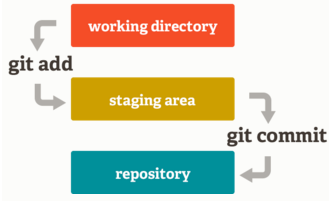
\includegraphics[width=.4\textwidth]{workflow}\\(from git-scm.com)
\end{center}
\end{frame}

% --- slide ---
\begin{frame}{Track a new file or record changes (stage)}
\begin{witemize}
\item Command: \code{git add <filename>}, \code{git add *}
\item SmartGit: select file(s) and click on the \code{Stage} button
\item You can unstage file(s) using the \code{git reset} command or the \code{Unstage} button
\end{witemize}
\end{frame}

% --- slide ---
\begin{frame}{Commit}
\begin{witemize}
\item Permanently\footnote{not really: you can use \code{git reset} in a dangerous manner to undo it.} record the changes
\item Command: \code{git commit -m "Commit message"}
\item SmartGit: click on the \code{Commit} button
\end{witemize}
\end{frame}

% --- slide ---
\begin{frame}{File status}
\begin{center}
  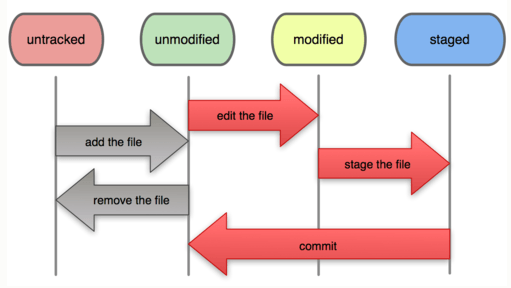
\includegraphics[width=0.8\textwidth]{filestatus}
\end{center}
\end{frame}

% --- slide ---
\begin{frame}{Pushing to a remote repo}
\begin{witemize}
\item Well-known remot repo hosts: GitHub, BitBucket, ...
\item If you did not clone a repo from a remote repo, then \code{origin} is not set.
\begin{itemize}
  \item Command: \code{git remote add origin URL}
  \item SmartGit: \code{Remote -> Add}
\end{itemize}
otherwise, \code{origin} is already set
\item Command to push a branch (say ``dev'')
\begin{itemize}
  \item Command: \code{git push origin dev}
  \item SmartGit: click on the \code{Push} button if \code{dev} is checked out; otherwise, right-click on the \code{dev} branch and select \code{Push}
\end{itemize}
\end{witemize}
\end{frame}

% --- slide ---
\begin{frame}{Fetch and Pull}
\begin{witemize}
\item Fetch: fetch remote changes, and bring my local repo up to date; no change to the working files
\item Pull: fetch and then bring (see next slide) the changes all the way to your working directly
\item Command:
\begin{itemize}
  \item Fetch (say origin): \code{git fetch origin}
  \item Pull: \code{git pull origin}
\end{itemize}
\item SmartGit: click on the \code{Pull} button and select \code{Pull} or \code{Fetch Only}
\end{witemize}
\end{frame}

% --- slide ---
\begin{frame}{Git data}
\begin{center}
  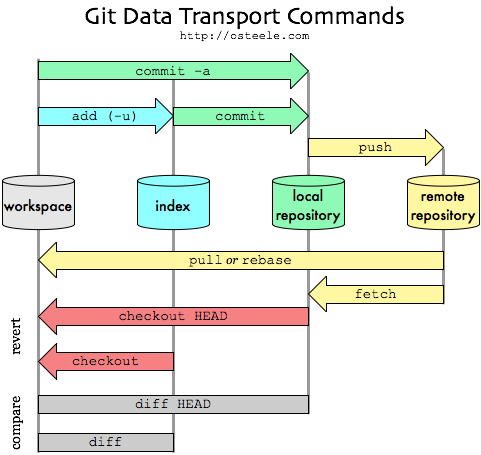
\includegraphics[width=0.8\textwidth]{data_transport}
\end{center}
\end{frame}

% --- slide ---
\begin{frame}{Pull: Merge vs Rebase}
\begin{witemize}
\item Two main ways to integrate changes from one branch to another
\item Merge: integrate diverged work history and keep work history unchanged (fast-forward, three-way merging, see \href{https://progit2.s3.amazonaws.com/en/2016-03-22-f3531/progit-en.1084.pdf}{GitPro})
\begin{center}
	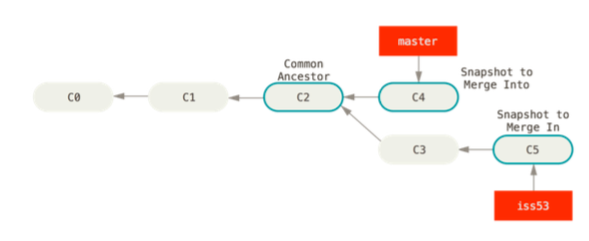
\includegraphics[width=0.8\textwidth]{merge1}
\end{center}
\begin{center}
	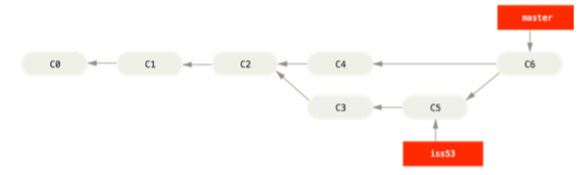
\includegraphics[width=0.8\textwidth]{merge2}
\end{center}
\end{witemize}
\end{frame}

% --- slide ---
\begin{frame}{Pull: Merge vs Rebase (cont'd)}
	\begin{witemize}
		\item Merge Command (in the above example):\\ \code{git checkout master\\git merge iss53}\\
		\code{git branch -d iss53} (delete merged branch)
		\item Merge SmartGit: \code{Branch -> Merge -> Select branch to be merged into current branch}
		
	\end{witemize}
\end{frame}

% --- slide ---
\begin{frame}{Pull: Merge vs Rebase (cont'd)}
	\begin{witemize}
		\item Rebase: takes all the changes that were commited on the current branch below the HEAD and reapply them on another one
		\item Changes work history, making it 'linear' 
		\begin{center}
			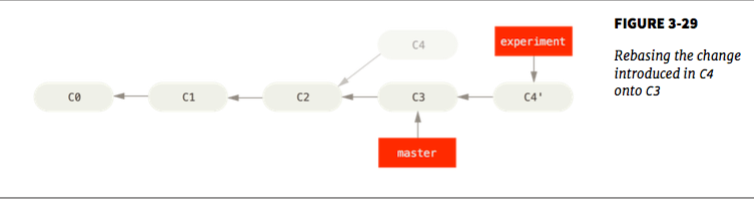
\includegraphics[width=1.0\textwidth]{rebase}
		\end{center}
		\item Note: \textbf{Do not rebase commits that exist outside your repository}
		
	\end{witemize}
\end{frame}

% --- slide ---
\begin{frame}{Pull: Merge vs Rebase (cont'd)}
	\begin{witemize}
		\item Rebase Command (in the above example): \\
		\code{git checkout experiment\\ git rebase master \\git checkout master}\\
		\code{git merge experiment} (fast-forward merge)
		\begin{center}
			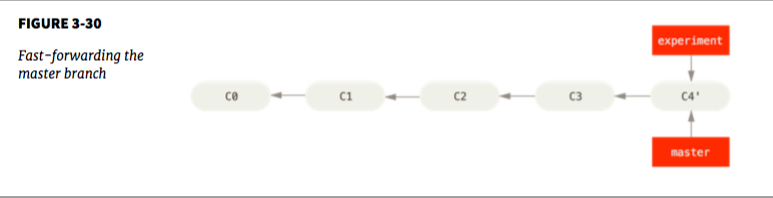
\includegraphics[width=1.0\textwidth]{rebase2}
		\end{center}
		
		
	\end{witemize}
\end{frame}

% --- slide ---
\begin{frame}{Pull: Merge vs Rebase (cont'd)}
	\begin{witemize}
		\item Rebase SmartGit: \code{Branch -> Rebase}
		\begin{itemize}
			\item \textbf{Rebase HEAD to} rebases ('moves') the commits below the HEAD to the selected commit
			\item \textbf{Rebase to HEAD} duplicates commits from a separate branch to the HEAD
			\item See \href{http://www.syntevo.com/doc/display/SG/Rebase}{\textit{here}} for illustrations
		\end{itemize}
		
	
		
		
	\end{witemize}
\end{frame}


% --- slide ---
\begin{frame}{Fork}
\begin{witemize}
\item  A fork is a copy of a repository
\item Most commonly, forks are used to either propose changes to someone else's project or to use someone else's project as a starting point for your own idea.
\item Two-step (say on GitHub): 
\begin{itemize}
	\item Navigate to the repository to be forked
	\item In the top-right corner of the page, click \textbf{Fork}
\end{itemize}
\end{witemize}
\end{frame}

% --- slide ---
\begin{frame}{Merge and Pull Request}
\begin{witemize}
\item  Merge a pull request into the upstream branch when work is completed. Anyone with push access to the repository can complete the merge
\item If the merge will not have any conflicts, you can merge the pull request online
\begin{center}
	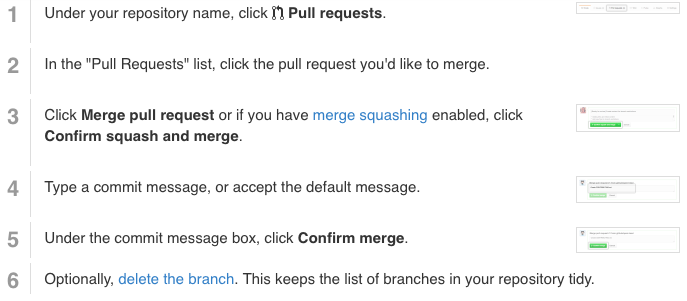
\includegraphics[width=1.0\textwidth]{pull_request}
\end{center}
\end{witemize}
\end{frame}

% --- slide ---
\begin{frame}{.gitignore}
\begin{witemize}
\item Specifies intentionally untracked files to ignore
\item Rules for patterns you can put in the \textbf{.gitignore} file are as follows:
\begin{itemize}
	\item Blank lines or lines starting with \# are ignored
	\item Standard glob patterns work
	\item You can start patterns with a forward slash to avoid recursivity
	\item You can end patterns with a forward slash to specify a directory
	\item You can negate a pattern by starting it with an exclamation point (!)
\end{itemize}
\item For more examples, see \href{https://progit2.s3.amazonaws.com/en/2016-03-22-f3531/progit-en.1084.pdf}{GitPro}
\end{witemize}
\end{frame}

% --- slide ---
\begin{frame}{(feel free to add other topics)}
\begin{witemize}
\item  
\end{witemize}
\end{frame}

\end{document}
